\documentclass{article}
\usepackage{amssymb,amsmath}
\usepackage{ifxetex,ifluatex}
\ifxetex
  \usepackage{fontspec,xltxtra,xunicode}
  \defaultfontfeatures{Mapping=tex-text,Scale=MatchLowercase}
\else
  \ifluatex
    \usepackage{fontspec}
    \defaultfontfeatures{Mapping=tex-text,Scale=MatchLowercase}
  \else
    \usepackage[utf8]{inputenc}
  \fi
\fi
\usepackage{ctable}
\usepackage{float} % provides the H option for float placement
\usepackage{graphicx}
% We will generate all images so they have a width \maxwidth. This means
% that they will get their normal width if they fit onto the page, but
% are scaled down if they would overflow the margins.
\makeatletter
\def\maxwidth{\ifdim\Gin@nat@width>\linewidth\linewidth
\else\Gin@nat@width\fi}
\makeatother
\let\Oldincludegraphics\includegraphics
\renewcommand{\includegraphics}[1]{\Oldincludegraphics[width=\maxwidth]{#1}}
\ifxetex
  \usepackage[setpagesize=false, % page size defined by xetex
              unicode=false, % unicode breaks when used with xetex
              xetex]{hyperref}
\else
  \usepackage[unicode=true]{hyperref}
\fi
\hypersetup{breaklinks=true, pdfborder={0 0 0}}
\setlength{\parindent}{0pt}
\setlength{\parskip}{6pt plus 2pt minus 1pt}
\setlength{\emergencystretch}{3em}  % prevent overfull lines
\setcounter{secnumdepth}{0}

\title{Descriptives}
\author{Rapport package team @ https://github.com/aL3xa/rapport}
\date{2011--04--26 20:25 CET}

\begin{document}
\maketitle

\subsection{Description}

This template will return descriptive statistics of a numerical, or a
frequency table of a categorical variable.

\subsubsection{\emph{gender} (``Gender'')}

The dataset has 709 observations with 709 valid values (missing: 0) in
\emph{gender} (``Gender''). This variable seems to be a factor.

\paragraph{Base statistics}

\ctable[pos = H, center, botcap]{lllll}
{% notes
}
{% rows
\FL
\textbf{gender} & \textbf{N} & \textbf{pct} & \textbf{cum.n} & \textbf{cum.pct}
\ML
male & 7344.00 & 60.93 & 7344.00 & 60.93
\\\noalign{\medskip}
female & 4709.00 & 39.07 & 12053.00 & 100.00
\LL
}

\paragraph{Barplot}

\begin{figure}[htbp]
\centering
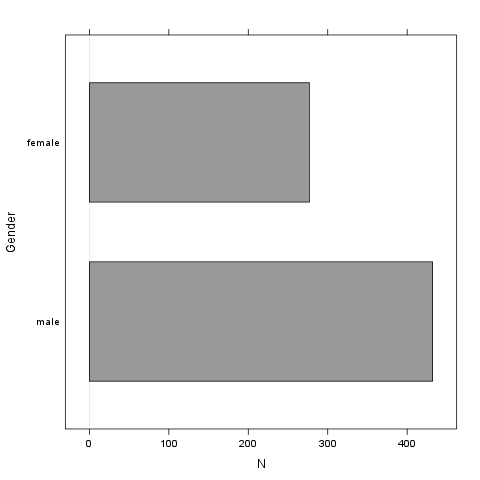
\includegraphics{7a6fc939fb3b30bcfda9ac649fd9d9af.png}
\caption{}
\end{figure}

It seems that the highest value is 2 which is exactly 2 times higher
than the smallest value (1).

\subsection{Description}

This template will return descriptive statistics of a numerical, or a
frequency table of a categorical variable.

\subsubsection{\emph{age}}

The dataset has 709 observations with 709 valid values (missing: 0) in
\emph{age}. This variable seems to be numeric.

\paragraph{Base statistics}

\ctable[pos = H, center, botcap]{llll}
{% notes
}
{% rows
\FL
\textbf{value} & \textbf{mean} & \textbf{sd} & \textbf{var}
\ML
(all) & 24.56 & 6.84 & 46.78
\LL
}

\paragraph{Histogram}

\begin{figure}[htbp]
\centering
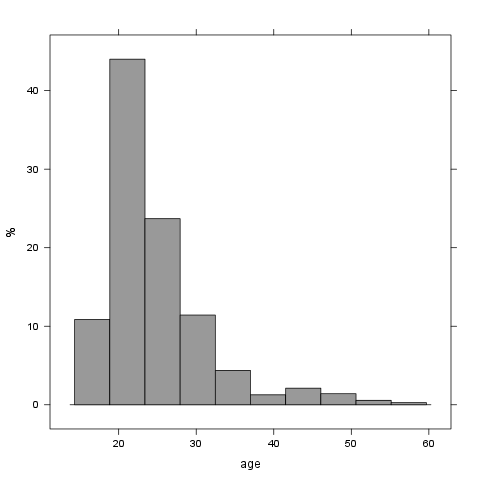
\includegraphics{ec60bf38bca8471ace82e1b6dfb6ae3f.png}
\caption{}
\end{figure}

It seems that the highest value is 58 which is exactly 3.625 times
higher than the smallest value (16).

\end{document}
